\section{Human Resource Management}
\label{sec:hrm}
\lhead{\thesection \space Human Resource Management}
Organize manage and lead the project team are processes of the Human Resource Management. Roles and responsibilities are assigned to people for a wealthy project outcome. People have different types of skill sets to achieve the best project outcome. Involving team members in the project planning and decision making process can be a beneficial task. Participation of team members during
planning adds their expertise to the process and strengthens their commitment to the project.

\subsection{Plan Human Resource Management}
Plan Human Resource Management is the process of identifying and documenting project roles, responsibilities,
required skills, reporting relationships, and creating a staffing management plan.

In the connected.Football project 4 project roles need to be assigned. Students have to choose a role that they will pursue throughout the entire project.
Sebastian is the lead software developer in this project
Marco is responsible for development and testing. Lucas is the scrum master and Patrick is the Product Manager. All these roles are more or less fictitious because everybody needs to code and have an understanding of all the parts in the project e.g. using Jira or create a chapter in the project plan. Guido Budziak operates as CEO and contact person where Thijs Dorssers is there to guide the project if students are working towards the wrong direction.

\begin{figure}[!ht]
  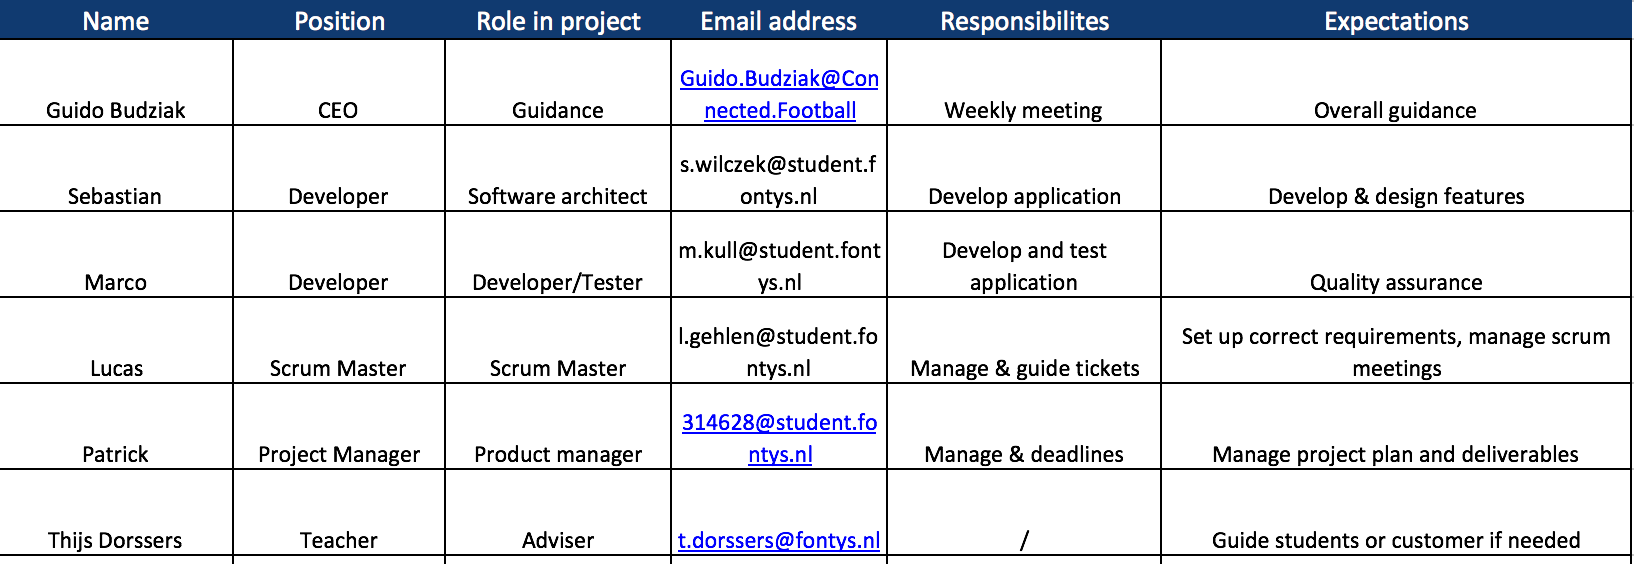
\includegraphics[width=\linewidth]{content/diagram/human/human_resc.png}
  \caption{Overview human resource management}
\end{figure}
\newpage

\subsection{Develop Project Team}
Develop Project Team is the process of improving competencies, team member interaction, and overall team
environment to enhance project performance. Over the 14 weeks students have to improve in certain areas. Lucas who is responsible for the scrum management has to study the tech stack with YouTube videos and the official documentation. Marco has to improve his knowledge in the area of web development and testing. Patrick in the role of a project manager should acquire skills to identify, build, maintain, motivate, lead, and inspire project teams
to achieve high team performance and to meet the project’s objectives. 
\subsection{Manage Project Team}
Manage Project Team is the process of tracking team member performance, providing feedback, resolving
issues, and managing team changes to optimize project performance. The project manager tries to identify lacks in knowledge areas and develops a strategy with the student to compensate the lack. Since there is no budget involved, students have to learn from free sources.